% !TeX spellcheck = cs_CZ
% \wikitextrule
\begin{mathexam}{Ověření Ohmová zákona}{exam076}
  Naměřili jsme následující hodnoty napětí na vodiči a jim odpovídající hodnoty proudu:
  
  \begin{center}
    \resizebox{1\textwidth}{!}{%
    \begin{tabular}{ccc|ccc}
      \hline
      měření & napětí [V] & proud [A]  & měření & napětí [V] & proud [A]    \\
      \hline
      1.     & \num{2.45} & \num{0.70} & 7.     & \num{7.42} & \num{2.17}   \\
      2.     & \num{4.33} & \num{1.22} & 8.     & \num{7.87} & \num{2.21}   \\
      3.     & \num{5.39} & \num{1.54} & 9.     & \num{8.14} & \num{2.34}   \\
      4.     & \num{5.76} & \num{1.66} & 10.    & \num{8.67} & \num{2.51}   \\
      5.     & \num{6.62} & \num{1.89} & 11.    & \num{9.12} & \num{2.53}   \\
      6.     & \num{7.05} & \num{2.00} & 12.    & \num{9.85} & \num{2.76}   \\
      \hline
    \end{tabular}}
  \end{center}

  {\centering
  \captionsetup{type=figure}
  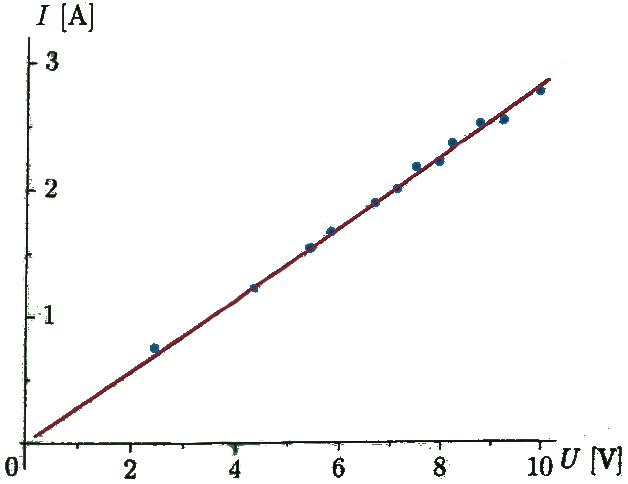
\includegraphics[width=0.8\linewidth]{mai_fig052.png}
  \captionof{figure}{Ověření Ohmová zákona lineární regresí.
  \cite[s.~263]{Musilova2009MA1}
  \label{mai:fig052}}
  \par}
  Pro odpor vychází \(R\doteq\SI{3.52}{\ohm}\). Součet čtverců odchylek přímky se směrnicí \(i/R
  = (1/\num{3.52})\Omega^{-1}\) od souboru bodů grafu je
  \begin{equation*}
    D(R) = \sum_{i=1}^{n}(U_i - R\cdot I_i)^2 \doteq\num{0.01},
  \end{equation*}
  \(\sigma(R) = \sqrt{D(R)/(n-1)}\doteq\sqrt{(\num{0.11}/11)}\doteq\num{0.03}\).  Graf přímky \(U
  = R\cdot I = \num{3.52}\cdot I\) proložené body je na obrázku \ref{mai:fig052}.
\end{mathexam}